\chapter{Realisierung der clientseitigen Implementierung als native App}
\label{cha:native-app}
Dieses Kapitel widmet sich der Implementierung der nativen Applikation. Im Kapitel \ref{cha:architektur} wurde eine grobe Übersicht zu der Umsetzung und der Funktionsweise dieser \ac{App} gegeben, die nun verfeinert wird.
Dabei werden folgend die verwendeten Komponenten und Techniken erläutert und die Zusammenhänge zwischen den Techniken dargestellt.
\section{Allgemeine Funktionsweise einer Android-App}
\label{sec:definition-android}
Grundlegend für die Entwicklung einer Android-App ist das Wissen über die Basis des Systems, auf dem entwickelt wird. 
Bei dem Betriebssystem \ac{Android} handelt es sich um eine Art eines \ac{monolithisch}en Multiuser-\ac{Linux}-Systems. \footcite{Android-Fundamentals}
Dieses Betriebssystem stellt die Hardwaretreiber zur Verfügung und führt die Prozessorganisation, sowie die Benutzer- und Speicherverwaltung durch.
Jede Applikation wird in einem eigenen Prozess gestartet. In diesem Prozess befindet sich eine \ac{Sandbox}, die eine virtuelle Maschine mit der Applikation ausführt. Die Kommunikation aus der Sandbox heraus kann nur über Schnittstellen des Betriebssystems geschehen. Diese Einschränkung sorgt für Sicherheit im System, da ein Prinzip der minimalen Rechte eingehalten wird. Demnach kann eine Applikation nur auf zugewiesene und freigegebene Ressourcen im System zugreifen. Ein weiterer Vorteil dieser internen Architektur liegt in der Robustheit des Systems. Wenn eine Applikation durch Fehler terminiert, wird nur der allokierte Prozess beendet und das Betriebssystem bleibt von diesem Problem unberührt. \footcite{Android-SystemPermissions}
Android-Applikationen werden in der Programmiersprache \ac{Java} geschrieben, mit einem Java-\ac{Compiler} kompiliert und dann von einem Cross-Assembler für die entsprechende \ac{VM} aufbereitet. Das Produkt ist ein ausführbares \ac{.apk}-Paket.\footcite[Seite 17-19]{Android-BeckerPant}
Im Folgenden werden die Android-Komponenten, die für die Umsetzung relevant sind, genauer betrachtet.
\subsection{User Interfaces}
\label{ssec:android-ui}
\textit{User Interfaces} sind die Bildschirmseiten der Android-Applikation. Über diese Seiten wird die Benutzerinteraktion geführt. Das \textit{User Interface} besteht aus zwei Arten von Elementen. Zum einen aus \textit{Views}, die es ermöglichen direkte Interaktionen mit dem Benutzer zu führen. Zu nennen sind dabei \textit{Buttons}, Textfelder und Checkboxen. Als zweites werden \textit{View Groups} verwendet, um \textit{Views} sowie andere \textit{View Groups} anzuordnen.
Das \textit{User Interface Layout} ist durch eine hierarchische Struktur gekennzeichnet. Zum Anlegen einer solchen Struktur gibt es verschiedene Möglichkeiten. Zum einen kann man ein \textit{View}-Objekt anlegen und darauf die Elemente platzieren. Aus Gründen der Performance und der Übersicht ist die Möglichkeit einer \ac{XML}-Datei jedoch zielführender. Aus den Knoten der erstellten Datei werden zur Laufzeit \textit{View}-Objekte erzeugt und angezeigt. Die erzeugten \textit{UIs} werden unter \textit{res/layout} im Android-Betriebssystem hinterlegt. Des Weiteren können Ressourcen in den \textit{UIs} verwendet werden. Unter Ressourcen versteht man Elemente, die zum Verzieren von Oberflächen verwendet werden können. Darunter fallen bespielsweise Grafiken oder \textit{Style-Sheets}, die über den jeweiligen Ressourcen-Schlüssel aufgerufen und verwendet werden.\footcite{Android-UI}

\subsection{Activities}
\label{ssec:android-activities}
\textit{Activities} gehören zu den App-Komponenten, da sie ein grundsätzlicher Bestandteil einer Applikation sind. Es gibt im Normalfall mehrere \textit{Activities} in einer App.

Die eigentlichen Aufgaben liegen in der Bereitstellung eines Fensters, das dann auf den Screen, der für die App vom Betriebssystem bereitgestellt wird, gelegt wird. Das Fenster ist im Anschluss für die Annahme von Benutzerinteraktionen bereit. Das Fenster wird mit Hilfe des Aufrufs \textit{SetContentView()} aufgerufen. Zur Benutzerinteraktion werden dann die bereits vorgestellten \textit{View}-Elemente verwendet. Die \textit{Activity} ist folgend für die Verarbeitung und Auswertung der Eingaben verantwortlich.

In jeder Applikation muss es eine \textit{MainActivity} geben, die beim Start der Applikation vom Android-Betriebssystem gestartet wird. Zudem muss eine \textit{Activity} im AndroidManifest mit dem Attribut \textit{Launcher} versehen werden, um diese dann als Einstiegspunkt aus dem Menü des Betriebssystems zu setzen. Dabei ist empfehlenswert, dass dieselbe \textit{Activity} sowohl das Main- als auch Launcher-Attribut erhält.

Diese Festlegungen müssen im Manifest hinterlegt werden. Das Manifest liegt im Root-Ordner der App und stellt dem Betriebssystem wichtige Informationen der Applikation zur Verfügung. Dieses Manifest wird vor Ausführung der App analysiert und ausgewertet. Darin kann beispielweise festgelegt werden, welche Komponenten oder anderen Applikationen auf entsprechende \textit{Activities} zugreifen dürfen. Wenn eine \textit{Activity} nicht von außerhalb der App erreicht werden soll, sollte kein Intent-Filter gesetzt werden, da demnach der genaue Name der \textit{Activity} zum Start bekannt sein muss. Diese Informationen sind jedoch nur in der gegenwärtigen App vorhanden.

Da eine App normalerweise aus mehreren \textit{Activities} besteht, müssen diese \textit{Activities} gestartet werden und untereinander kommunizieren. \textit{Activities} starten sich gegenseitig, weshalb der Aufruf einer \textit{Activity} aus einer anderen erfolgt. Um eine neue \textit{Activity} starten zu können, ist ein Intent von Nöten.
Ein Intent ist ein Nachrichtenobjekt innerhalb von Android, welches zur Kommunikation zwischen App-Komponenten verwendet wird. In diesem Fall zwischen zwei \textit{Activities}. Zur Erstellung benötigt es den Namen der zu startenden Komponente, um eine Verbindung dorthin aufbauen zu können, und eine \textit{Action}, die ausgeführt werden soll. Zudem können Daten übergeben werden, die anschließend als Datenpakete mit dem Aufruf der Komponente mitgegeben werden. Diese Daten sind dann in der gestarteten Komponente aus dem dort vorhandenen Intent auslesbar. Zusätzlich gibt es die Möglichkeit Aktionen vom Betriebssystem ausführen zu lassen. Beispielsweise kann man ein \textit{Intent} mit der Aktion zum Starten des Email-Programms übergeben und die entsprechend im Betriebssystem hinterlegte Applikation zum schreiben von Emails wird geöffnet.

Eine \textit{Activity} kann drei Stati in einem \textit{Lifecycle} einnehmen. Zum einen kann die \textit{Activity} im Status \textit{Resumed} - oft auch \textit{Running} genannt - sein und damit momentan im User-Fokus stehen, also im Vordergrund der App sein und die Interaktionen entgegennehmen. Des Weiteren kann eine \textit{Activity} pausieren, wenn eine andere im User-Fokus steht. Dabei ist der \textit{View} der betrachteten \textit{Activity} jedoch immer noch teilweise sichtbar, da der darüberliegende \textit{View} zu Beispiel nicht den gesamten Bildschirm in Anspruch nimmt. Anders verhält es sich, wenn der \textit{View} der betrachteten \textit{Activity} komplett überdeckt ist. Dann befindet sich die \textit{Activity} nämlich im Status \textit{Stopped}. Sowohl im Status \textit{Stopped} als auch im Status \textit{Paused} lebt die \textit{Activity} noch. Das bedeutet, dass das \textit{Activity}-Objekt zusammen mit allen Objekt-Stati und Memberinformationen im Arbeitsspeicher liegt. Der einzige Unterschied dieser beiden Stati liegt darin, dass eine \textit{Activity} im Status \textit{Paused} noch eine Verbindung zum \textit{WindowManager} besitzt, die im Status \textit{Stopped} nicht mehr vorhanden ist. Gemeinsam haben diese beiden Stati jedoch noch, dass sie bei mangelndem Arbeitsspeicher vom Betriebssystem zerstört werden können. 

%Lifecycle-Bild
\begin{figure}[h]
\centering
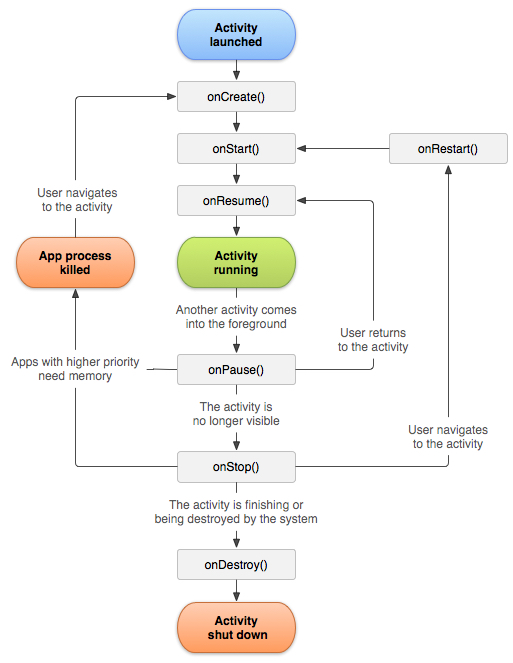
\includegraphics[width=0.8\linewidth]{Bilder/Android-ActivityLifecycle}
\caption{Android Activity-Lifecycle}
Quelle: https://developer.android.com/guide/components/activities.html
\label{pic:androidActivityLifecycle}
\end{figure}

Die Ausführung der internen Methoden einer \textit{Activity} ist abhängig von den Eingaben des Benutzers. Dabei durchläuft jede \textit{Activity} ihren \textit{Lifecycle}, der in Abbildung~\ref{pic:androidActivityLifecycle} dargestellt ist. Darin ist zu erkennen, dass zuerst die \textit{OnCreate()}-Methode aufgerufen wird. Darin werden alle essentiellen Initialisierungen gemacht und der \textit{View} aufgerufen. Nachfolgend werden \textit{OnStart()} und \textit{OnResume()} durchlaufen bis die \textit{Activity} den User-Fokus wieder verliert, jedoch der \textit{View} noch sichtbar ist. In dem Moment wird die \textit{OnPause()}-Methode ausgeführt, um Benutzereingaben gegebenenfalls speichern zu können, denn in diesem Zustand ist es in seltenen Fällen möglich, dass der Status - wie oben erklärt - durch das Betriebssystem zerstört wird. Kehrt der Benutzer zurück, wird \textit{OnResume()} wieder aufgerufen, sonst \textit{OnStop()}, um auch dort aufgenommene Daten persitieren zu können. Von dort gibt es zwei verschiedene Rücksprung-Möglichkeiten. Zum einen könnte der Fall eintreten, dass die Daten der \textit{Activity} aus dem Arbeitsspeicher gelöscht wurden, die \textit{Activity} jedoch noch einmal aufgerufen wird. In diesem Fall startet die \textit{Activity} wieder von vorn. Eine weitere Möglichkeit ist die Rückkehr des Benutzers zu der \textit{Activity}. Dabei werden dann die Methoden \textit{OnRestart()} und \textit{OnStart()} aufgerufen.

Zusammenfassend lässt sich daraus ableiten, dass die Persistierung von Eingaben in den Methoden \textit{OnPause()}, \textit{OnStop()} und \textit{OnDestroy()} durchgeführt werden sollten, da diese Zustände zerstört werden können. Die weiteren Methoden sollten aus Performancegründen jedoch minimal und agil gehalten werden.



\subsection{Services}
\label{ssec:android-services}

\subsection{Threading/Asynchronität}
\label{ssec:android-threading-async}

\section{Was ist XAMARIN?}
\label{sec:defintion-xamarin}

\subsection{Multiplattform-Unterstützung}
\label{ssec:xamarin-multiplattform}

\subsection{Besonderheiten der Android-Umsetzung}
\label{ssec:xamarin-android}
Man muss Activities nicht manuell im Manifest eintragen -> macht XAMARIN für einen!

\section{Eigene Umsetzung}
\label{sec:nat-umsetzung}

\subsection{Anlegen der Layouts}
\label{ssec:nat-layouts}

\subsection{Konnektivität zum Server}
\label{ssec:nat-konnektivität}

\subsection{Lokale Datenbank}
\label{ssec:nat-db}

\subsection{Umsetzung des Caches}
\label{ssec:nat-cache}
